\chapter{传播效应：等离子体、尘埃和引力透镜}
\label{chap:14}

\begin{chapteropening}
从源到望远镜的路上，光子会穿过自由电子、湍流磁化等离子体、尘埃颗粒、地球大气和弯曲时空。传播过程会改写事件表中的到达时间、频率、偏振、方向和计数相关。冷等离子体给出 \(\nu^{-2}\) 色散和 Faraday 旋转，湍流给出散射尾和闪烁，尘埃给出消光、红化和偏振选择，引力透镜复制路径并产生放大和延迟。NE2001 与 YMW16 电子密度模型、局域 FRB 的 baryon census、星际散射综述、尘埃消光和透镜时间延迟宇宙学给出了这些效应的典型量级 \citep{2002astro.ph..7156C,2017ApJ...835...29Y,2020Natur.581..391M,1977ARA&A..15..479R,1990ARA&A..28..561R,2004ApJ...605..759B,1989ApJ...345..245C,1999PASP..111...63F,1964MNRAS.128..295R,1964MNRAS.128..307R,2016A&ARv..24...11T}。
\end{chapteropening}

\section{为什么传播要当成带记忆的通道}

传播效应最容易被误当成“观测以后再扣掉的前景”。这在平均光度或平均颜色问题中有时够用，但在本书关心的事件表、相干性和强度相关里不够。原因是传播不只是乘上一个常数；它会把一个源端光子的标签重新写一遍。频率标签决定色散延迟，偏振标签决定 Faraday 旋转，角位置标签被散射和透镜混合，到达时间标签会被多条路径复制出回声。因此更好的第一步不是问“源本来多亮”，而是问“源端场经过怎样的通道才变成探测器事件”。

先看场的版本。若把两个偏振、多个频率通道和多个空间模式合并成一个向量，传播可以写成
\begin{equation}
  {\bf a}_{\rm out}(\omega,\hat{\bf n})
  =
  {\bf S}(\omega,\hat{\bf n})\,{\bf a}_{\rm src}(\omega,\hat{\bf n})
  +{\bf n}_{\rm fg}(\omega,\hat{\bf n}) ,
  \label{eq:ch14-channel-frequency}
\end{equation}
\begin{formulaexplain}[公式 (14.1) 解读]
\({\bf a}_{\rm out}\) 是到达观测端的场模，\({\bf a}_{\rm src}\) 是源端场模，\({\bf S}\) 是传播矩阵，\({\bf n}_{\rm fg}\) 是前景和探测噪声。这条式子把传播看成一个线性通道：介质既能旋转、混合或衰减信号，也会加入额外背景。
\end{formulaexplain}
其中 \({\bf a}_{\rm src}\) 是源发出的湮灭算符或经典场模振幅，\({\bf S}\) 是传播矩阵，\({\bf n}_{\rm fg}\) 代表前景热辐射、天空背景和探测链噪声。若介质只吸收而不散射，\({\bf S}\) 近似对角；若存在 Faraday 旋转，\({\bf S}\) 在两个线偏振之间转动；若存在散射或透镜，\({\bf S}\) 同时混合方向和到达时间。时间域里同一件事写成
\begin{equation}
  E_{{\rm out},i}(t)
  =
  \sum_j\int h_{ij}(t-t')\,E_{{\rm src},j}(t')\,{\rm d}t'
  + n_i(t) ,
  \label{eq:ch14-channel-time}
\end{equation}
\begin{formulaexplain}[公式 (14.2) 解读]
\(E_{{\rm out},i}\) 是第 \(i\) 个观测通道的电场，\(h_{ij}\) 是从源通道 \(j\) 到观测通道 \(i\) 的响应函数，\(n_i\) 是噪声。积分表示传播有记忆：一个源端时刻的光可以被延迟、展宽后贡献到许多观测时刻。
\end{formulaexplain}
\(i,j\) 标记偏振、望远镜、像或频率通道。\(h_{ij}\) 的单位取决于电场归一化；在脉冲和强度相关分析中，最常用的是它的时间宽度、峰值延迟和不同通道之间的相对相位。地球质心改正、钟差、大气延迟和仪器电子延迟也属于这个响应的一部分；脉冲星计时模型把这些项分开到 ns 级，是高时间分辨天文学中最成熟的校准例子之一 \citep{2006MNRAS.372.1549E}。

事件表中一个光子候选可写为 \((t_q,\nu_q,p_q,{\bf x}_q,w_q)\)。\(t_q\) 是到达时刻，单位 s；\(\nu_q\) 是频率，单位 Hz；\(p_q\) 是偏振通道；\({\bf x}_q\) 是像素、基线或望远镜编号；\(w_q\) 是质量权重。传播模型给出源端标签到观测标签的映射。色散主要改变 \(t_q(\nu_q)\)，Faraday 旋转改变 \(p_q(\lambda_q^2)\)，散射把一个窄脉冲变成带长尾的到达时间分布，尘埃改变不同 \(\lambda_q\) 的接受概率，透镜把一个源事件复制到多个 \({\bf x}_q\) 和多个 \(t_q\)。

传播误差预算常被这些量级支配。银河系高纬 DM 常为 \(30-100\,{\rm pc\,cm^{-3}}\)，FRB 可到 \(10^3-10^4\,{\rm pc\,cm^{-3}}\)，它来自脉冲到达时间随 \(\nu^{-2}\) 的斜率。普通星际介质的 RM 多为 \(1-10^2\,{\rm rad\,m^{-2}}\)，磁化致密环境可到 \(10^4-10^5\,{\rm rad\,m^{-2}}\)，它来自线偏振角随 \(\lambda^2\) 的斜率。散射展宽 \(\tau_{\rm sc}\) 可从 \(\mu{\rm s}\) 到 s，低频端增长很快，同一 DM 下也可相差数量级。光学消光在高银纬常小于 \(0.1\) mag，在银盘和分子云中可为数 mag。透镜延迟的范围更宽：行星或恒星质量透镜可在 \(\mu{\rm s}\)-ms，星系强透镜常在天到年。

\section{色散和 Faraday 旋转怎样量出电子与磁场}

本章先从最干净的传播效应开始：冷等离子体不会把一个脉冲完全随机化，而是让低频光子稍微晚到，并让线偏振角随 \(\lambda^2\) 旋转。重要的是这两个量都来自“斜率”。动态谱里的到达时间对 \(\nu^{-2}\) 的斜率给 DM；偏振角对 \(\lambda^2\) 的斜率给 RM。只要先抓住这个读法，下面的常数和单位换算就有了清楚的物理位置。

冷等离子体的折射率在 \(\omega\gg\omega_p\) 时近似为
\begin{equation}
  n(\omega)\simeq 1-\frac{\omega_p^2}{2\omega^2},
  \qquad
  \omega_p^2=\frac{4\pi n_e e^2}{m_e}.
  \label{eq:ch14-plasma-index}
\end{equation}
\begin{formulaexplain}[公式 (14.3) 解读]
\(n(\omega)\) 是折射率，\(\omega_p\) 是等离子体频率，\(n_e\) 是自由电子密度。电子越多，\(\omega_p\) 越大，低频电磁波的群速度偏离 \(c\) 越明显，因此会产生频率依赖的到达时间。
\end{formulaexplain}
\(n_e\) 是自由电子数密度，单位 \({\rm cm^{-3}}\)；银河系温暖电离介质常为 \(10^{-2}-10^{-1}\,{\rm cm^{-3}}\)，HII 区和 FRB 局部环境可高出很多。由群速度积分得到色散量
\begin{equation}
  {\rm DM}=\int n_e\,{\rm d}l ,
  \label{eq:ch14-dm-definition}
\end{equation}
\begin{formulaexplain}[公式 (14.4) 解读]
DM 是视线方向自由电子柱密度，\({\rm d}l\) 是路径长度元。这条式子说明 DM 不是局部密度，而是整条传播路径上电子数密度的累积。
\end{formulaexplain}
\({\rm d}l\) 用 pc，因而 DM 的单位是 \({\rm pc\,cm^{-3}}\)。两个射频通道之间的冷等离子体延迟为
\begin{equation}
  \Delta t_{\rm DM}
  =
  4.148808\,{\rm ms}\,
  {\rm DM}
  \left[
  \left(\frac{\nu_1}{\rm GHz}\right)^{-2}
  -
  \left(\frac{\nu_2}{\rm GHz}\right)^{-2}
  \right].
  \label{eq:ch14-dispersion-delay}
\end{equation}
\begin{formulaexplain}[公式 (14.5) 解读]
\(\Delta t_{\rm DM}\) 是两个频率通道的到达时差，\(\nu_1,\nu_2\) 是观测频率。延迟正比于 DM，且随 \(\nu^{-2}\) 改变；这就是射电脉冲动态谱中最容易识别的弯曲扫频轨迹。
\end{formulaexplain}
若 \({\rm DM}=300\,{\rm pc\,cm^{-3}}\)，\(0.6\) GHz 相对 \(1.4\) GHz 的延迟约 \(2.9\) s；同一个事件在 \(1.2\) 与 \(1.5\) GHz 之间只差约 \(0.36\) s。射电脉冲和 FRB 的搜索通常先在一组 trial DM 上去色散，再找峰值信噪比。通道宽度 \(\Delta\nu\) 也会带来通道内展宽，量级为
\begin{equation}
  \Delta t_{\rm chan}
  \simeq
  8.3\,\mu{\rm s}\,
  \left(\frac{{\rm DM}}{{\rm pc\,cm^{-3}}}\right)
  \left(\frac{\Delta\nu}{\rm MHz}\right)
  \left(\frac{\nu}{\rm GHz}\right)^{-3}.
  \label{eq:ch14-channel-smearing}
\end{equation}
\begin{formulaexplain}[公式 (14.6) 解读]
\(\Delta t_{\rm chan}\) 是一个有限频率通道内部的色散展宽，\(\Delta\nu\) 是通道宽度。它告诉我们：即使整体去色散正确，通道太宽也会把微秒级结构平均掉。
\end{formulaexplain}
这条式子的左边可从动态谱中每个频率通道的脉冲宽度估计；右边显示高 DM、宽通道和低频观测会直接把微秒结构洗掉。

\begin{figure}[tbp]
\centering
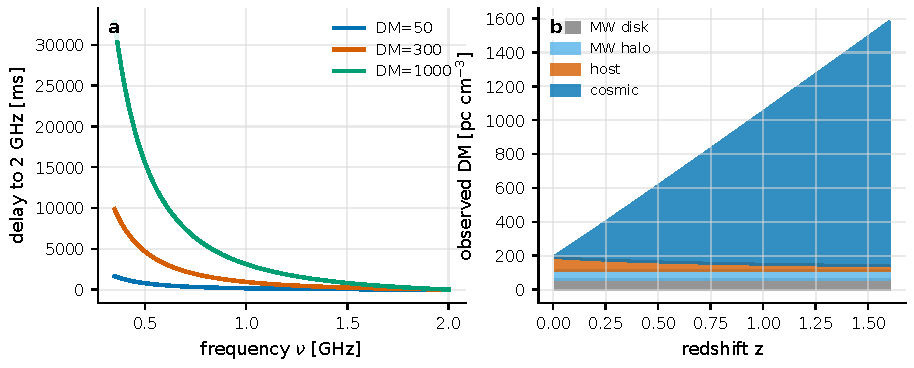
\includegraphics[width=0.94\linewidth]{figures/generated/chapter_14/ch14_dispersion_delay.pdf}
\caption{冷等离子体色散和 FRB 的 DM 预算。左图把到达时间延迟画成频率函数，参考频率为 \(2\,{\rm GHz}\)；低频端的 \(\nu^{-2}\) 斜率使 DM 很容易从宽带动态谱中估计。右图把一个局域 FRB 的观测 DM 拆成银河系盘、银晕、宿主星系和宇宙学等离子体贡献；宿主项因宇宙学时间膨胀按 \((1+z)^{-1}\) 进入观测值，宇宙学项在 \(z\lesssim1\) 近似随红移增长。}
\label{fig:ch14-dispersion}
\end{figure}

银河系电子密度远非一个常数。NE2001 把厚盘、薄盘、旋臂、局部空洞和团块组合起来，用脉冲星 DM、独立距离和散射数据约束参数；YMW16 更新了厚盘、薄盘、旋臂、银河中心和 Magellanic Clouds/IGM 处理，用来把脉冲星或 FRB 的银河系 DM 转换成距离或前景估计 \citep{2002astro.ph..7156C,2017ApJ...835...29Y}。高银纬视线的银河系盘 DM 常为 \(30-100\,{\rm pc\,cm^{-3}}\)，银晕贡献常取 \(50-100\,{\rm pc\,cm^{-3}}\) 的数量级；靠近银盘、HII 区或超新星遗迹时，局部结构会比平滑模型更重要。

宇宙学 FRB 常写成
\begin{equation}
  {\rm DM}_{\rm FRB}
  =
  {\rm DM}_{\rm MW,ISM}
  +{\rm DM}_{\rm MW,halo}
  +{\rm DM}_{\rm cosmic}(z)
  +\frac{{\rm DM}_{\rm host}}{{1+z}} .
  \label{eq:ch14-frb-dm-budget}
\end{equation}
\begin{formulaexplain}[公式 (14.7) 解读]
\({\rm DM}_{\rm FRB}\) 被拆成银河系盘、银晕、宇宙学等离子体和宿主星系四部分。这个预算式的意义是把一次 FRB 的总色散量变成沿途不同结构的电子柱密度账本。
\end{formulaexplain}
宿主星系项除以 \(1+z\)，因为观测到的频率和时间间隔已经被红移拉伸。均匀宇宙近似下
\begin{equation}
  {\rm DM}_{\rm cosmic}(z)
  =
  \frac{3cH_0\Omega_b f_{\rm IGM}}{8\pi Gm_p}
  \int_0^z
  \frac{f_e(z')(1+z')}{\sqrt{\Omega_m(1+z')^3+\Omega_\Lambda}}
  {\rm d}z' ,
  \label{eq:ch14-cosmic-dm}
\end{equation}
\begin{formulaexplain}[公式 (14.8) 解读]
\({\rm DM}_{\rm cosmic}\) 是宇宙学大尺度结构贡献，积分变量 \(z'\) 沿红移累加自由电子。前面的系数给出平均重子密度，积分核描述膨胀宇宙中电子数和路径长度如何随红移变化。
\end{formulaexplain}
\(\Omega_b\) 是重子密度参数，\(f_{\rm IGM}\) 是进入弥散 IGM 的重子比例，\(f_e\) 是每个重子的自由电子数。局域 FRB 样本给出的 \({\rm DM}_{\rm cosmic}\)-\(z\) 关系已经能测量宇宙重子含量；实际散布来自 cosmic web 的非均匀性，常用 \(\sigma_{\rm DM}\simeq F z^{-1/2}\) 的形式描述，\(F\sim0.1-0.4\) 对应不同 baryon feedback 和 halo gas 分布 \citep{2020Natur.581..391M,2014ApJ...790..101S}。

磁化等离子体使左右圆偏振的相速度不同，线偏振角随波长平方旋转：
\begin{equation}
  \psi(\lambda)=\psi_0+{\rm RM}\,\lambda^2 ,
  \label{eq:ch14-rm-angle}
\end{equation}
\begin{formulaexplain}[公式 (14.9) 解读]
\(\psi\) 是线偏振角，\(\psi_0\) 是本征偏振角，RM 是旋转量。偏振角对 \(\lambda^2\) 的斜率就是 RM，因此多频偏振观测能直接读出磁化等离子体的累积效应。
\end{formulaexplain}
\begin{equation}
  {\rm RM}
  =
  0.812
  \int
  \left(\frac{n_e}{{\rm cm^{-3}}}\right)
  \left(\frac{B_\parallel}{\mu{\rm G}}\right)
  \left(\frac{{\rm d}l}{\rm pc}\right)
  {\rm rad\,m^{-2}} .
  \label{eq:ch14-rm-definition}
\end{equation}
\begin{formulaexplain}[公式 (14.10) 解读]
RM 是 \(n_e\) 与视线磁场 \(B_\parallel\) 的路径积分。它不同于 DM：DM 只数电子，RM 还保留磁场方向信息，所以磁场反转会让 RM 互相抵消。
\end{formulaexplain}
\(B_\parallel\) 是指向观测者的磁场分量。若 DM 和 RM 主要来自同一区域，视线平均磁场可估为
\begin{equation}
  \langle B_\parallel\rangle
  \simeq
  1.232\,\mu{\rm G}\,
  \frac{{\rm RM}/{\rm rad\,m^{-2}}}{{\rm DM}/{\rm pc\,cm^{-3}}}.
  \label{eq:ch14-bfield-rm-dm}
\end{equation}
\begin{formulaexplain}[公式 (14.11) 解读]
\(\langle B_\parallel\rangle\) 是由 RM/DM 推出的电子加权平均磁场。这个估计只有在 RM 和 DM 来自同一段介质时才有直接物理含义。
\end{formulaexplain}
这不是一个普适磁场测量：若 RM 来自磁化宿主星系而 DM 大部分来自 IGM，式 \eqref{eq:ch14-bfield-rm-dm} 会低估局部磁场；若视线中有磁场反转，RM 会相互抵消而 DM 不会。星系团和星系际介质的 RM 研究常把这类退化与 X 射线气体密度、射电 halo 和背景源网格结合起来处理 \citep{2002ARA&A..40..319C}。

\begin{figure}[tbp]
\centering
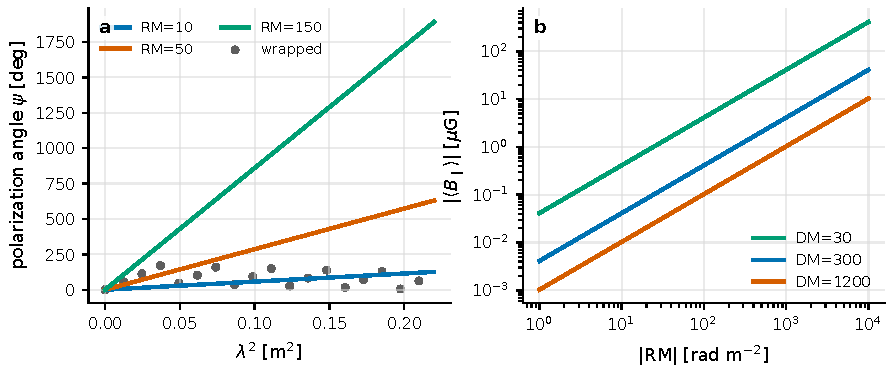
\includegraphics[width=0.94\linewidth]{figures/generated/chapter_14/ch14_faraday_rotation.pdf}
\caption{Faraday 旋转的两个读法。左图展示 \(\psi=\psi_0+{\rm RM}\lambda^2\) 的线性关系；黑点显示实际偏振角只在模 \(\pi\) 意义下测得，窄带数据容易出现缠绕歧义。右图把 \(\langle B_\parallel\rangle=1.232\,{\rm RM}/{\rm DM}\) 画成 RM 的函数；同一 RM 在低 DM 介质中代表更强的平均磁场。}
\label{fig:ch14-faraday}
\end{figure}

\section{散射、闪烁和尘埃怎样重排到达概率}

色散和 Faraday 旋转主要改变不同频率、不同偏振之间的相对相位或延迟；散射和尘埃更进一步，直接改变光子到达某个时间、方向、波长和偏振通道的概率。星际电子密度不是平滑函数。湍流中的小尺度起伏把波前打皱，结果是角展宽、脉冲展宽和强度闪烁。若源的本征强度是 \(I_{\rm src}(t)\)，单个薄屏近似常把观测脉冲写成卷积
\begin{equation}
  I_{\rm obs}(t)
  =
  \int I_{\rm src}(t')\,P(t-t')\,{\rm d}t',
  \qquad
  P(t)=\frac{1}{\tau_{\rm sc}}\exp\!\left(-\frac{t}{\tau_{\rm sc}}\right)H(t),
  \label{eq:ch14-scattering-convolution}
\end{equation}
\begin{formulaexplain}[公式 (14.12) 解读]
\(I_{\rm obs}\) 是观测强度，\(I_{\rm src}\) 是源端强度，\(P(t)\) 是散射到达时间核。单侧指数核表示光只能被延迟到达，不能提前到达，所以窄脉冲会变成长尾。
\end{formulaexplain}
\(P(t)\) 是一侧指数散射核，\(H(t)\) 是 Heaviside 函数。真实视线可有多个屏、各向异性散射和有限源尺寸，指数尾只是最常用的低阶模型。散射时间常写成
\begin{equation}
  \tau_{\rm sc}\propto \nu^{-\alpha},
  \label{eq:ch14-scattering-power}
\end{equation}
\begin{formulaexplain}[公式 (14.13) 解读]
\(\tau_{\rm sc}\) 是散射展宽时间，\(\alpha\) 是频率指数。指数越大，低频散射尾增长越快；这也是低频脉冲搜索容易丢失窄结构的原因。
\end{formulaexplain}
Kolmogorov 湍流薄屏给 \(\alpha\simeq4.4\)，多频脉冲星样本给出的经验平均更接近 \(\alpha=3.9\pm0.2\)，并且在固定 DM 下有超过一个数量级的散布 \citep{1977ARA&A..15..479R,1990ARA&A..28..561R,1995ApJ...443..209A,2004ApJ...605..759B}。常用经验式为
\begin{equation}
  \log_{10}\!\left(\frac{\tau_{\rm sc}}{{\rm ms}}\right)
  =
  -6.46
  +0.154\log_{10}{\rm DM}
  +1.07(\log_{10}{\rm DM})^2
  -3.86\log_{10}\!\left(\frac{\nu}{\rm GHz}\right),
  \label{eq:ch14-bhat-scattering}
\end{equation}
\begin{formulaexplain}[公式 (14.14) 解读]
这是一条经验散射关系，把 \(\tau_{\rm sc}\) 与 DM 和观测频率 \(\nu\) 联系起来。它适合做数量级预估，但真实视线的湍流结构会带来很大的散布。
\end{formulaexplain}
其中 DM 用 \({\rm pc\,cm^{-3}}\)。这条式子适合估计数量级，不适合替代每条视线的散射测量。对 \({\rm DM}=300\,{\rm pc\,cm^{-3}}\)，它给出 \(1.4\,{\rm GHz}\) 下约 ms 级的展宽；降到 \(600\,{\rm MHz}\) 时，展宽可增加到十几 ms 或更高。动态谱中的去相关带宽 \(\Delta\nu_d\) 与时间展宽近似满足
\begin{equation}
  \tau_{\rm sc}\simeq \frac{C_1}{2\pi\Delta\nu_d},
  \label{eq:ch14-decorrelation-bandwidth}
\end{equation}
\begin{formulaexplain}[公式 (14.15) 解读]
\(\Delta\nu_d\) 是闪烁去相关带宽，\(C_1\) 是几何相关的常数。时间展宽越长，频域中的相关带宽越窄；时间和频率是同一个多路径延迟分布的两种投影。
\end{formulaexplain}
\(C_1\) 是与几何和散射谱有关的常数，通常为 1 附近。强散射时，\(\Delta\nu_d\) 很窄，宽带平均会抹平闪烁；弱散射时，闪烁图样随时间和频率漂移，反而能测量屏速度、屏距离和源角尺寸。

\begin{figure}[tbp]
\centering
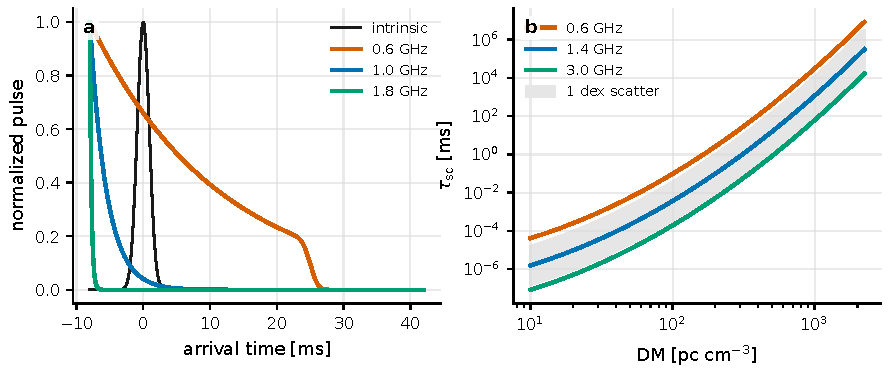
\includegraphics[width=0.94\linewidth]{figures/generated/chapter_14/ch14_scattering_broadening.pdf}
\caption{星际散射把短脉冲变成带长尾的到达时间分布。左图把一个窄高斯脉冲与一侧指数核卷积；频率越低，\(\tau_{\rm sc}\propto\nu^{-4}\) 使尾部越长。右图使用经验关系画出 \(\tau_{\rm sc}\) 随 DM 和频率的变化；灰色带表示固定 DM 下常见的数量级散布。}
\label{fig:ch14-scattering}
\end{figure}

等离子体还可以像透镜一样折射。横向电子柱密度梯度给出频率依赖的相位屏，低频光线偏折更强，强度可出现 caustic、multiple imaging 和 narrow-band 放大。高斯 plasma lens、FRB 宿主星系 plasma structures，以及非均匀等离子体中的引力透镜修正都表明，去掉 \(\nu^{-2}\) 色散以后，剩余结构仍可能来自传播过程 \citep{1998ApJ...496..253C,2010MNRAS.404.1790B,2014MNRAS.437.2180E,2017ApJ...842...35C}。在银河中心方向，毫米 VLBI 也要面对强散射屏；Sgr A* 的事件视界尺度成像需要同时处理本征结构、散射模糊和时间变化 \citep{2008Natur.455...78D,2022ApJ...930L..14E,2022ApJ...930L..15E}。

尘埃对光学和红外光子的影响更像一个带波长和偏振选择的损耗通道。通量关系为
\begin{equation}
  F_{\lambda,{\rm obs}}
  =
  F_{\lambda,{\rm int}}\,10^{-0.4A_\lambda},
  \label{eq:ch14-extinction-flux}
\end{equation}
\begin{formulaexplain}[公式 (14.16) 解读]
\(F_{\lambda,{\rm int}}\) 是本征通量，\(F_{\lambda,{\rm obs}}\) 是消光后的通量，\(A_\lambda\) 是波长相关消光。星等中的 \(0.4A_\lambda\) 转成指数衰减，表示尘埃按波长选择性吸收和散射光子。
\end{formulaexplain}
\(A_\lambda\) 的单位是 mag。选择性消光写成
\begin{equation}
  E(B-V)=A_B-A_V,
  \qquad
  R_V=\frac{A_V}{E(B-V)}.
  \label{eq:ch14-rv-definition}
\end{equation}
\begin{formulaexplain}[公式 (14.17) 解读]
\(E(B-V)\) 是蓝光和可见光消光差，\(R_V\) 把总消光与选择性红化相连。\(R_V\) 越大，消光曲线通常越灰，说明较大尘埃颗粒贡献更重要。
\end{formulaexplain}
银河系平均 \(R_V\simeq3.1\)，弥散 ISM 常在 \(2.5-3.5\) 附近，致密云中可到 \(5\) 以上，表示大颗粒使消光更灰。Cardelli-Clayton-Mathis 消光律把红外、光学和紫外平均曲线写成一个 \(R_V\) 参数族；Fitzpatrick 给出了实际视线中仍然存在的明显散布，尤其是 \(2175\,\text{\AA}\) bump 和 far-UV rise 的强弱 \citep{1989ApJ...345..245C,1999PASP..111...63F,2003ARA&A..41..241D}。若用平均消光律修正一个 \(E(B-V)=0.2\) mag 的蓝色源，紫外误差达到 \(0.1\) mag 并不奇怪；对偏振角、颜色温度和瞬变源早期谱能量分布，这已经是主要系统误差。

非球形尘埃颗粒在磁场中部分取向，会让通过的星光线偏振。常用 Serkowski 关系为
\begin{equation}
  \frac{P(\lambda)}{P_{\max}}
  =
  \exp\!\left[-K\ln^2\!\left(\frac{\lambda_{\max}}{\lambda}\right)\right],
  \label{eq:ch14-serkowski}
\end{equation}
\begin{formulaexplain}[公式 (14.18) 解读]
\(P(\lambda)\) 是尘埃造成的线偏振度，\(P_{\max}\) 是峰值，\(\lambda_{\max}\) 是峰值波长，\(K\) 控制曲线宽度。它把偏振随波长的形状和尘埃颗粒尺寸、取向环境联系起来。
\end{formulaexplain}
\(\lambda_{\max}\) 通常接近 \(0.55\,\mu{\rm m}\)，\(P_{\max}\) 的经验上限约为 \(9E(B-V)\%\)。这个上限不是每条视线都会达到；它受颗粒形状、取向效率、磁场方向变化和多云层叠加影响 \citep{1975ApJ...196..261S,2015ARA&A..53..501A}。尘埃散射还会把短暂爆发变成光回声或 X 射线 halo。若尘埃屏位于源到观测者距离的分数 \(x\)，散射角为 \(\theta\)，几何延迟近似
\begin{equation}
  \Delta t_{\rm dust}
  \simeq
  \frac{D_s}{2c}\frac{x}{1-x}\theta^2 ,
  \label{eq:ch14-dust-delay}
\end{equation}
\begin{formulaexplain}[公式 (14.19) 解读]
\(\Delta t_{\rm dust}\) 是尘埃散射造成的几何延迟，\(D_s\) 是源距离，\(x\) 是尘埃屏的相对位置，\(\theta\) 是散射角。延迟随 \(\theta^2\) 增长，因此角分辨光回声能反推出尘埃几何。
\end{formulaexplain}
\(D_s\) 是源距离。对银河系源，角秒级散射可给出小时到天的延迟；对银河系外源，尘埃几何和角分辨率要一起进入模型。

\begin{figure}[tbp]
\centering
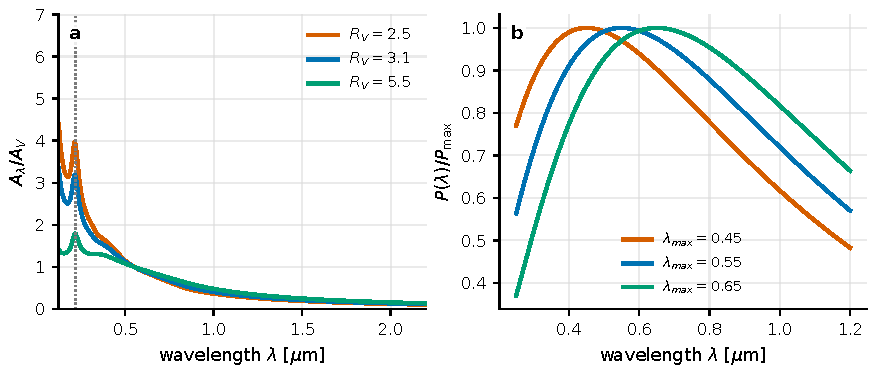
\includegraphics[width=0.94\linewidth]{figures/generated/chapter_14/ch14_dust_extinction_polarization.pdf}
\caption{尘埃改变光子的颜色、通量和偏振。左图是 CCM 平均消光曲线，\(R_V\) 越大，光学到近红外消光越灰；\(0.2175\,\mu{\rm m}\) 附近的紫外 bump 是小颗粒和碳质材料的重要诊断。右图是 Serkowski 偏振曲线，\(\lambda_{\max}\) 的移动反映颗粒尺寸和取向环境变化。}
\label{fig:ch14-dust}
\end{figure}

\section{引力透镜怎样把一条路径变成多条路径}

等离子体和尘埃来自真实介质；引力透镜来自弯曲时空。它不改变光子的频率色散关系，但改变路径、方向和到达时间。对事件表来说，透镜的核心动作很简单：一个源事件可以变成多个像、多个到达时刻和多个放大权重。薄透镜近似下
\begin{equation}
  {\boldsymbol\beta}
  =
  {\boldsymbol\theta}
  -
  {\boldsymbol\alpha}({\boldsymbol\theta}),
  \label{eq:ch14-lens-equation}
\end{equation}
\begin{formulaexplain}[公式 (14.20) 解读]
\({\boldsymbol\beta}\) 是源的真实角位置，\({\boldsymbol\theta}\) 是像位置，\({\boldsymbol\alpha}\) 是约化偏折角。透镜方程说明观测到的像不是源的直接方向，而是被质量分布偏折后的解。
\end{formulaexplain}
\({\boldsymbol\beta}\) 是真实源位置，\({\boldsymbol\theta}\) 是像位置，\({\boldsymbol\alpha}\) 是约化偏折角，三者常用角单位 rad 或 arcsec。点质量透镜的 Einstein 角为
\begin{equation}
  \theta_E
  =
  \left(
  \frac{4GM}{c^2}
  \frac{D_{ls}}{D_lD_s}
  \right)^{1/2}.
  \label{eq:ch14-einstein-angle}
\end{equation}
\begin{formulaexplain}[公式 (14.21) 解读]
\(\theta_E\) 是 Einstein 角，\(M\) 是透镜质量，\(D_l,D_s,D_{ls}\) 是角直径距离组合。它给出强透镜和微透镜的自然角尺度，也决定多像分离的量级。
\end{formulaexplain}
\(D_l\)、\(D_s\)、\(D_{ls}\) 是角直径距离。\(M=1\,M_\odot\)、银河系尺度几何给出 mas 量级的 \(\theta_E\)；星系质量透镜给出 arcsec 量级的多像分离。放大率为
\begin{equation}
  \mu
  =
  \frac{1}{\det(\partial{\boldsymbol\beta}/\partial{\boldsymbol\theta})},
  \label{eq:ch14-magnification}
\end{equation}
\begin{formulaexplain}[公式 (14.22) 解读]
\(\mu\) 是放大率，分母是从像平面到源平面的 Jacobian 行列式。行列式趋近零时，像面积被强烈拉伸，caustic 附近就会出现高放大。
\end{formulaexplain}
caustic 附近 \(|\mu|\) 可很大，但有限源尺寸、微透镜、尘埃和时间采样会限制实际可观测峰值。

到达时间由 Fermat 势控制：
\begin{equation}
  t({\boldsymbol\theta},{\boldsymbol\beta})
  =
  \frac{D_{\Delta t}}{c}
  \left[
  \frac{1}{2}|{\boldsymbol\theta}-{\boldsymbol\beta}|^2
  -
  \psi({\boldsymbol\theta})
  \right],
  \qquad
  D_{\Delta t}
  =
  (1+z_l)\frac{D_lD_s}{D_{ls}} .
  \label{eq:ch14-fermat-delay}
\end{equation}
\begin{formulaexplain}[公式 (14.23) 解读]
\(t({\boldsymbol\theta},{\boldsymbol\beta})\) 是相对到达时间，括号内第一项是几何路径差，\(\psi\) 是引力势延迟，\(D_{\Delta t}\) 是时间延迟距离。像的位置对应 Fermat 势的驻点。
\end{formulaexplain}
\(\psi\) 是二维透镜势，\(D_{\Delta t}\) 是时间延迟距离。两幅像之间的观测延迟为
\begin{equation}
  \Delta t_{AB}
  =
  \frac{D_{\Delta t}}{c}\,
  \Delta\phi_{AB}.
  \label{eq:ch14-time-delay-distance}
\end{equation}
\begin{formulaexplain}[公式 (14.24) 解读]
\(\Delta t_{AB}\) 是两幅像的到达时间差，\(\Delta\phi_{AB}\) 是 Fermat 势差。观测延迟乘上透镜模型后给出 \(D_{\Delta t}\)，因此可以约束 \(H_0\)。
\end{formulaexplain}
星系强透镜的 \(\Delta t_{AB}\) 常为天到月，少数系统可到年；它只占 \(D_{\Delta t}/c\) 的 \(10^{-11}\) 左右，因此透镜势、外部收敛、质量片退化和光变曲线采样都会直接进入 \(H_0\) 误差预算。Refsdal 首先指出多像时间延迟可测 \(H_0\)；现代 time-delay cosmography 依赖多年监测、高分辨成像、透镜星系速度弥散和环境建模 \citep{1964MNRAS.128..295R,1964MNRAS.128..307R,1986ApJ...310..568B,2016A&ARv..24...11T}。

\begin{figure}[tbp]
\centering
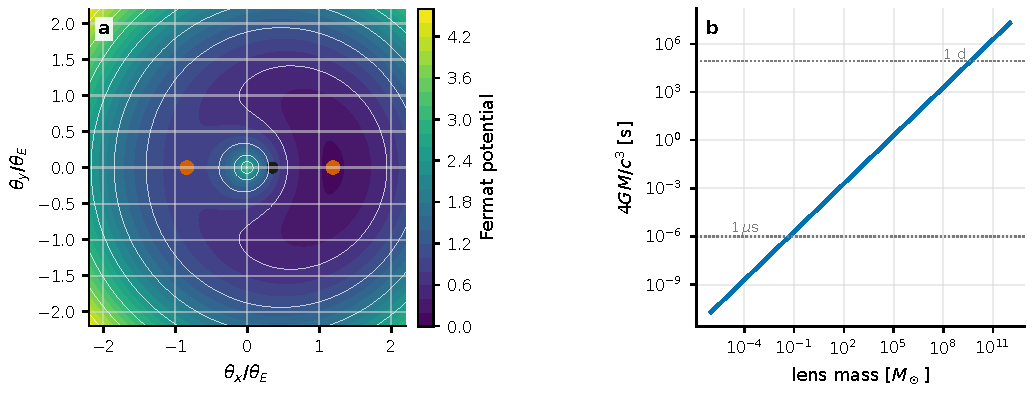
\includegraphics[width=0.94\linewidth]{figures/generated/chapter_14/ch14_lensing_time_delay.pdf}
\caption{强透镜的两个尺度。左图是点质量透镜的 Fermat 到达时间面，黑点是源位置，两个橙点是像位置；像出现在到达时间面的驻点。右图给出 \(4GM/c^3\) 的基本延迟尺度：恒星质量透镜对应微秒到毫秒，星系和星系团透镜自然进入天到年的时间域。}
\label{fig:ch14-lensing}
\end{figure}

当波长不能忽略时，几何光学的“多条光线”要改成波的衍射积分。对引力波透镜常用无量纲频率
\begin{equation}
  w
  =
  \frac{8\pi GM(1+z_l)f}{c^3}.
  \label{eq:ch14-wave-lensing-w}
\end{equation}
\begin{formulaexplain}[公式 (14.25) 解读]
\(w\) 是波动光学透镜的无量纲频率，\(M\) 是透镜质量，\(f\) 是波频率。\(w\) 比较的是波的周期和透镜引起的时间尺度：大 \(w\) 近似几何光学，小 \(w\) 必须考虑衍射。
\end{formulaexplain}
\(w\gg1\) 时回到几何光学，多像可分开并产生相干干涉条纹；\(w\lesssim1\) 时衍射抹平 caustic，放大率不再能用几何像简单相加。频域波形写为
\begin{equation}
  \tilde h_L(f)=F(f)\,\tilde h(f),
  \label{eq:ch14-wave-amplification}
\end{equation}
\begin{formulaexplain}[公式 (14.26) 解读]
\(\tilde h(f)\) 是未透镜波形，\(\tilde h_L(f)\) 是透镜后的频域波形，\(F(f)\) 是复放大因子。它同时包含振幅放大和相位延迟，所以可以产生频率依赖的干涉结构。
\end{formulaexplain}
\(F(f)\) 是复放大因子。若两条路径延迟为 \(\Delta t\)，干涉条纹的频率间隔约为
\begin{equation}
  \Delta f \simeq \frac{1}{\Delta t}.
  \label{eq:ch14-lensing-fringe-spacing}
\end{equation}
\begin{formulaexplain}[公式 (14.27) 解读]
\(\Delta f\) 是频域条纹间距，\(\Delta t\) 是两条路径的时间延迟。路径延迟越长，频域振荡越密；这把时间结构转写成谱中的干涉条纹。
\end{formulaexplain}
例如 \(\Delta t=2\,{\rm ms}\) 时，条纹间隔约 \(500\,{\rm Hz}\)。对电磁光学频率，普通恒星或星系质量透镜通常 \(w\) 极大，几何光学非常好；对 LISA 频段引力波和 \(10^6-10^9M_\odot\) 透镜，波动光学效应可以进入观测带 \citep{2003ApJ...595.1039T}。

\begin{figure}[tbp]
\centering
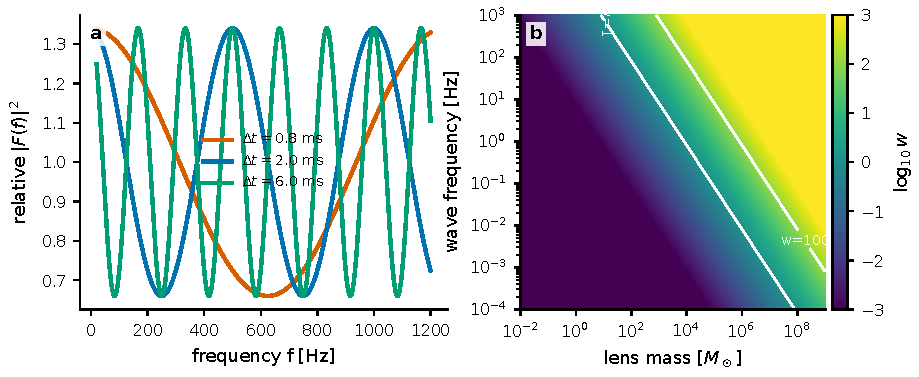
\includegraphics[width=0.94\linewidth]{figures/generated/chapter_14/ch14_wave_lensing_interference.pdf}
\caption{波动光学透镜把时间延迟变成频域条纹。左图画出不同路径延迟下的相对放大因子振荡，\(\Delta f\simeq1/\Delta t\)。右图给出 \(w=8\pi GMf/c^3\) 的量级；白线 \(w=1\) 附近是衍射与几何光学的过渡，\(w=100\) 以上通常可把像当成独立路径处理。}
\label{fig:ch14-wave-lensing}
\end{figure}

\section{相关函数和 cosmic Bell 的边界在哪里}

前面几节把传播写成对单个事件标签的改写。最后要回到本书主线：相关函数。多路径传播会重排强度相关，因为观测到的涨落不一定来自源端同一时刻；它可能是同一个源端结构沿不同路径晚到、早到或被放大后的叠加。若透镜或散射在观测带内可近似为若干离散路径，
\begin{equation}
  h(t)=\sum_i \sqrt{\mu_i}\,e^{i\varphi_i}\delta(t-t_i),
  \label{eq:ch14-multipath-impulse}
\end{equation}
\begin{formulaexplain}[公式 (14.28) 解读]
\(h(t)\) 是多路径脉冲响应，\(\mu_i\) 是第 \(i\) 条路径放大率，\(\varphi_i\) 是相位，\(t_i\) 是到达延迟。每个 delta 函数代表一条可分辨路径。
\end{formulaexplain}
\(\mu_i\) 是第 \(i\) 条路径的放大率，\(\varphi_i\) 是相位，\(t_i\) 是到达时间。若相位在带宽或源尺寸上被平均掉，观测强度近似
\begin{equation}
  I_{\rm obs}(t)
  =
  \sum_i \mu_i I_{\rm src}(t-t_i).
  \label{eq:ch14-multipath-intensity}
\end{equation}
\begin{formulaexplain}[公式 (14.29) 解读]
\(I_{\rm obs}\) 是观测强度，\(I_{\rm src}\) 是源端强度。相位平均后，不同路径的强度按放大率加权相加，因此一个源端变化会在多个延迟处重复出现。
\end{formulaexplain}
对强度涨落 \(\delta I=I-\langle I\rangle\)，自相关函数
\begin{equation}
  C_{\rm obs}(\tau)
  =
  \left\langle
  \delta I_{\rm obs}(t)\,
  \delta I_{\rm obs}(t+\tau)
  \right\rangle
  =
  \sum_{ij}\mu_i\mu_j
  C_{\rm src}\!\left(\tau+t_i-t_j\right)
  \label{eq:ch14-correlation-echo}
\end{equation}
\begin{formulaexplain}[公式 (14.30) 解读]
\(C_{\rm obs}\) 是观测强度自相关，\(C_{\rm src}\) 是源端自相关。双重求和表示每一对路径都会贡献一个相关回声，回声位置由两条路径的延迟差决定。
\end{formulaexplain}
会在 \(\tau=t_j-t_i\) 附近出现回声结构。这个关系只在源本身有可测快速结构、传播路径稳定、观测时间覆盖足够长、背景和选择函数已经建模时有用。热光的 \(g^{(2)}(0)\) 峰、脉冲星 giant pulse 的微结构、FRB 的窄带 scintillation 和透镜多像延迟都可落入这个框架，但它们的相干时间、带宽和统计分布不同；相关峰本身还不足以确定物理来源。

传播效应也定义了 cosmic Bell test 的适用边界。实验室 Bell 检验使用纠缠光子对，两个站点选择测量设置 \(a,a'\) 和 \(b,b'\)，CHSH 组合为
\begin{equation}
  S
  =
  E(a,b)+E(a,b')+E(a',b)-E(a',b'),
  \qquad
  |S|\le 2
  \label{eq:ch14-chsh}
\end{equation}
\begin{formulaexplain}[公式 (14.31) 解读]
\(S\) 是 CHSH 组合，\(E(a,b)\) 是给定测量设置下的相关期望值。局域隐变量模型要求 \(|S|\le2\)；cosmic Bell 实验用天文光子选择设置，是为了把可能共同原因推到更早的宇宙时刻。
\end{formulaexplain}
是局域隐变量模型的上限。cosmic Bell 实验用银河系恒星或高红移类星体光子实时决定 \(a\) 和 \(b\)，目的是把可能共同原因推到更早的时空区域，而不是证明天体光子本身处在纠缠态。Milky Way stars 版本使用星光颜色产生设置并处理大气延迟、探测噪声和错误设置概率；quasar 版本进一步把自由选择漏洞的共同过去推到宇宙早期 \citep{2017PhRvL.118f0401H,2018PhRvL.121h0403R}。这类实验检验的是因果结构：天文光子可以参与量子基础实验的设置选择，但传播中的吸收、红化、色散和仪器延迟要逐项进入实验时序。

\begin{figure}[tbp]
\centering
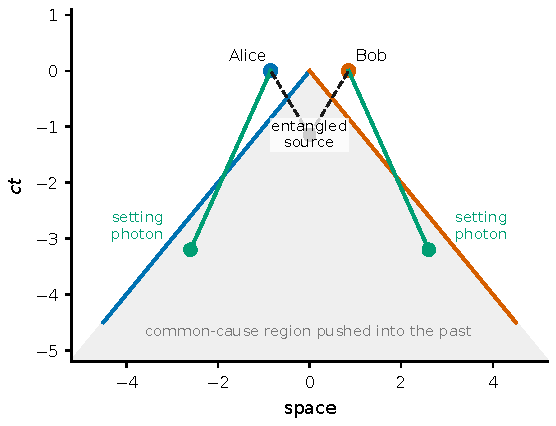
\includegraphics[width=0.72\linewidth]{figures/generated/chapter_14/ch14_cosmic_bell_lightcones.pdf}
\caption{Cosmic Bell 实验的光锥结构。纠缠源在本地实验中发出光子对，Alice 和 Bob 的测量设置由远处恒星或类星体光子决定；这些设置光子的发射事件越早、方向分离越大，可能共同原因被排除的时空区域越大。图中灰区表示被推向过去的共同原因区域，实际实验还要加入大气传播、探测器响应和电子延迟。}
\label{fig:ch14-cosmic-bell}
\end{figure}

普通传播效应给出了新物理搜索的误差地板。轴子样粒子可让光子在磁场中转化，宇宙双折射会旋转偏振，暗物质小结构可改写透镜放大率和时间延迟；这些解释需要先和等离子体、尘埃、透镜和仪器项放在同一个模型中比较。若剩余信号同时经得起时间、频率、偏振和角位置检验，才有资格作为新物理候选。

